\section{Manual}
Manual类提供一个如何使用该程序的提示信息。

\section{HashFactory}
HashFactory类中存在三个函数。

printInfo()用来输出我们已有的Hash赋值方式。

ChooseHash()用来通过传参的方式来获取进行那种Hash方式。

剩下的为具体Hash赋值的实现。

\section{Detect}
Detect类为一个抽象类,其中含有一个startDetect()的纯虚函数,用来在积累中重新定义。之所以将Detect设为抽象类是因为,在以后的扩展中,可能会加入一些新的检查相似度的方法,这为以后的发展起了很大作用。

\section{similarity}
similarity类是Detect类的一个派生类,其重新定义了startDetect()函数。它用来实现相似度检测的一个类,首先他会从一个Reader的函数接口获取一个文件被预处理之后的一个个单词,接下来会将这些单词赋予Hash值,另外在similarity.h中,提供了一个Sig结构,该结构用来存储一个文件的Hash值构成的特征信息。在将所有的文件都经过处理得到其Sig结构之后,我们调用compare()函数来获取其相似度。

\section{使用及效果}
\begin{center}
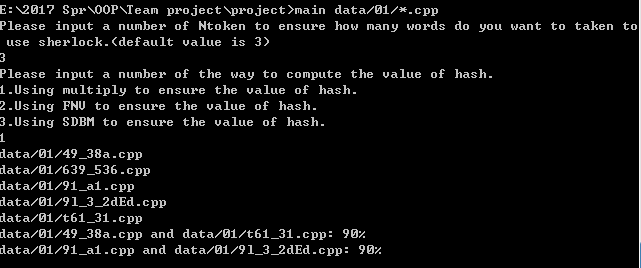
\includegraphics{command.PNG}
\end{center}

我们通过命令行参数传入所要进行检测的文件名,然后在提示信息下,我们输入一个数字代表一次性对几个连续的单词进行赋予特征值(Hash),然后第二个提示信息我们将输入一个代表Hash赋值方式的数字,目前为止,我们可以提供三种不同Hash赋值的方式,可以多次进行检测,增加准确度。接下来的几行则是输出所有待检测文件的文件名,最后会输出相似度。

因为是抄袭检测,所以我们设置了一个参数——20\%,如果相似度低于20%的话,则不会输出其相似度的具体值,代表其抄袭的可能性较低。

\newpage
